To test our program we did some captures in different moments of the day to see what we are able to 
understand from them.


\subsection{Sonos speakers interconnected via WiFi}
 A capture that brought something interesting to our attention is the \texttt{Filtered
\_capture\_SONOS\_WEDNESDAY\_MILAN.pcapng} done in Milan on a wednesday morning. Thanks to the vendor 
classification we spotted four MAC addresses related to \textbf{Sonos} devices, a vendor famous for
wireless home sound systems in which multiple speakers are interconnected using WiFi. In this capture,
we found four different devices which produced most of the traffic: the \textit{MAC} addresses of the Sonos 
devices are:
\begin{itemize}
    \item \textbf{00:0e:58:c2:48:5f}
    \item \textbf{00:0e:58:c2:48:05}
    \item \textbf{00:0e:58:67:a3:e9}
    \item \textbf{00:0e:58:f4:7a:83}
\end{itemize}
As we can see in Figure \ref{fig:Sonos_traffic}, there are a lot of traffic spikes mainly due to the
communication between those speakers. The highest peak is the combination of the communication between
the Sonos devices and other communication flows.
\begin{figure}[h]
    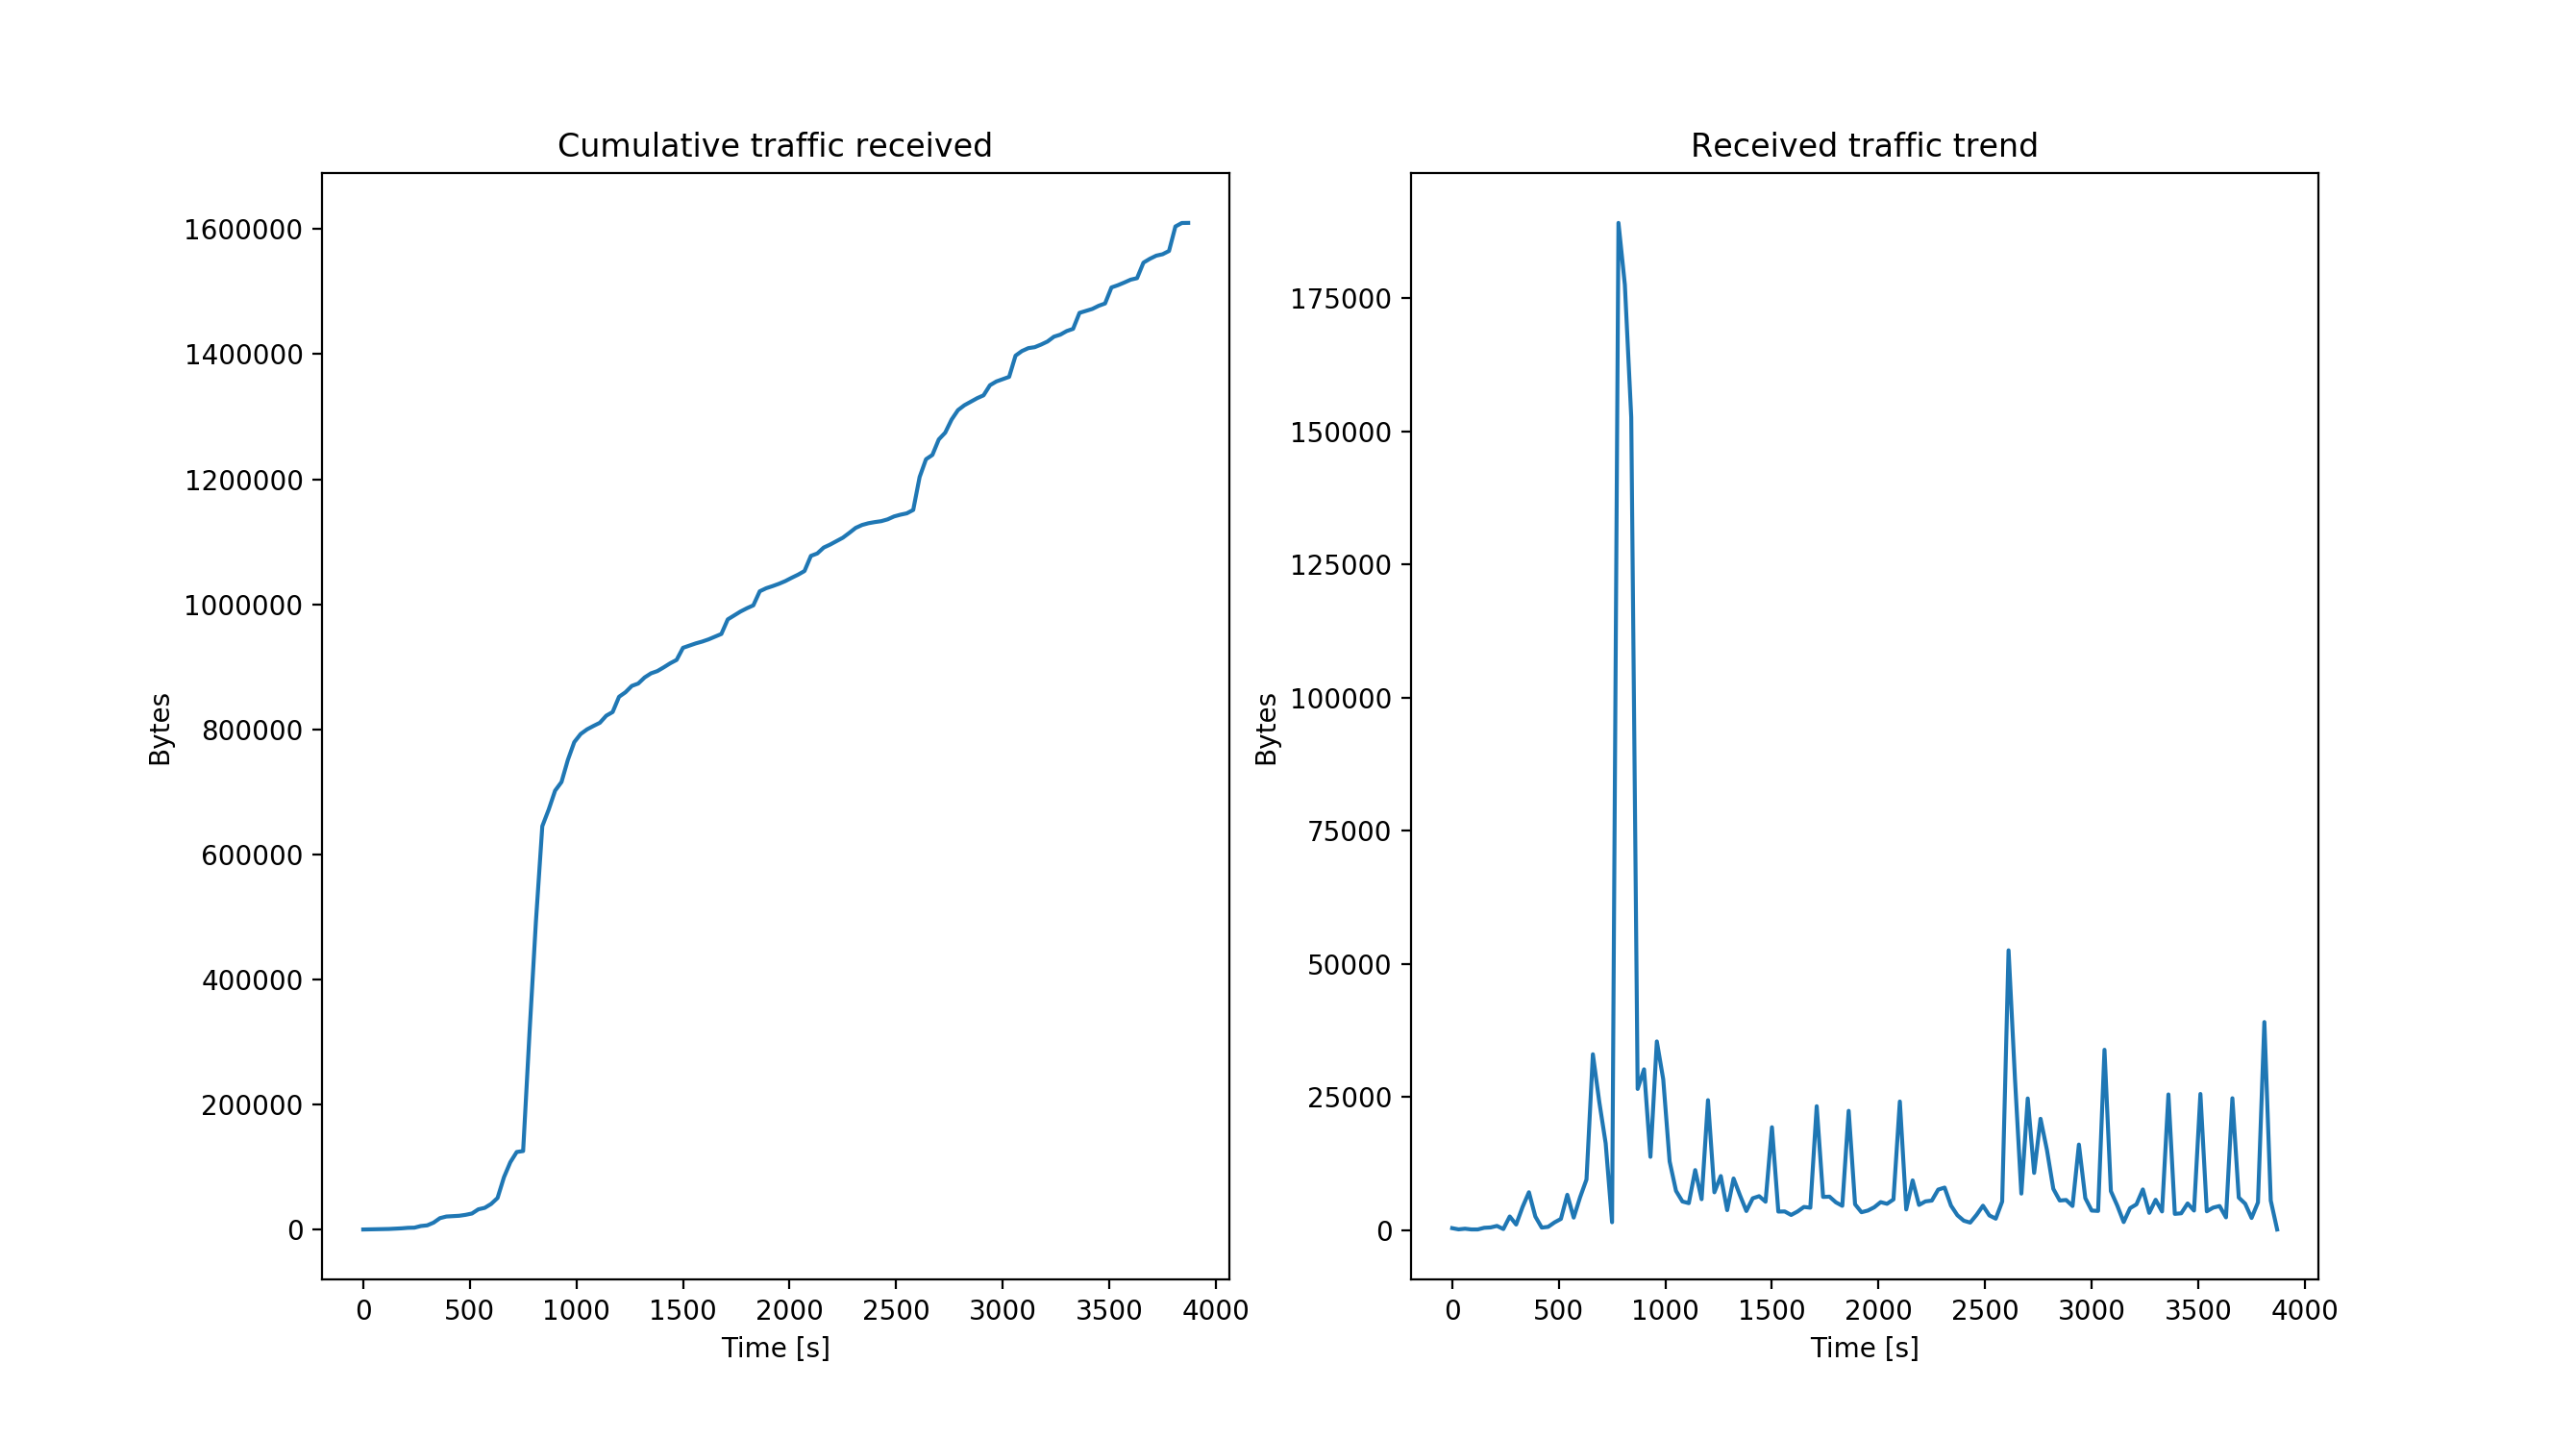
\includegraphics[width=\textwidth]{Graphs/SONOS_cum_in_traffic.png}
    \caption{Sonos input traffic graphs}
    \label{fig:Sonos_traffic}
\end{figure}
\\
To further show how many packets the Sonos devices exchanged we can see that three out of the four
devices are at the top spots of the following graph (Figure \ref{fig:Sonos_packets}).
\begin{figure}[h]
    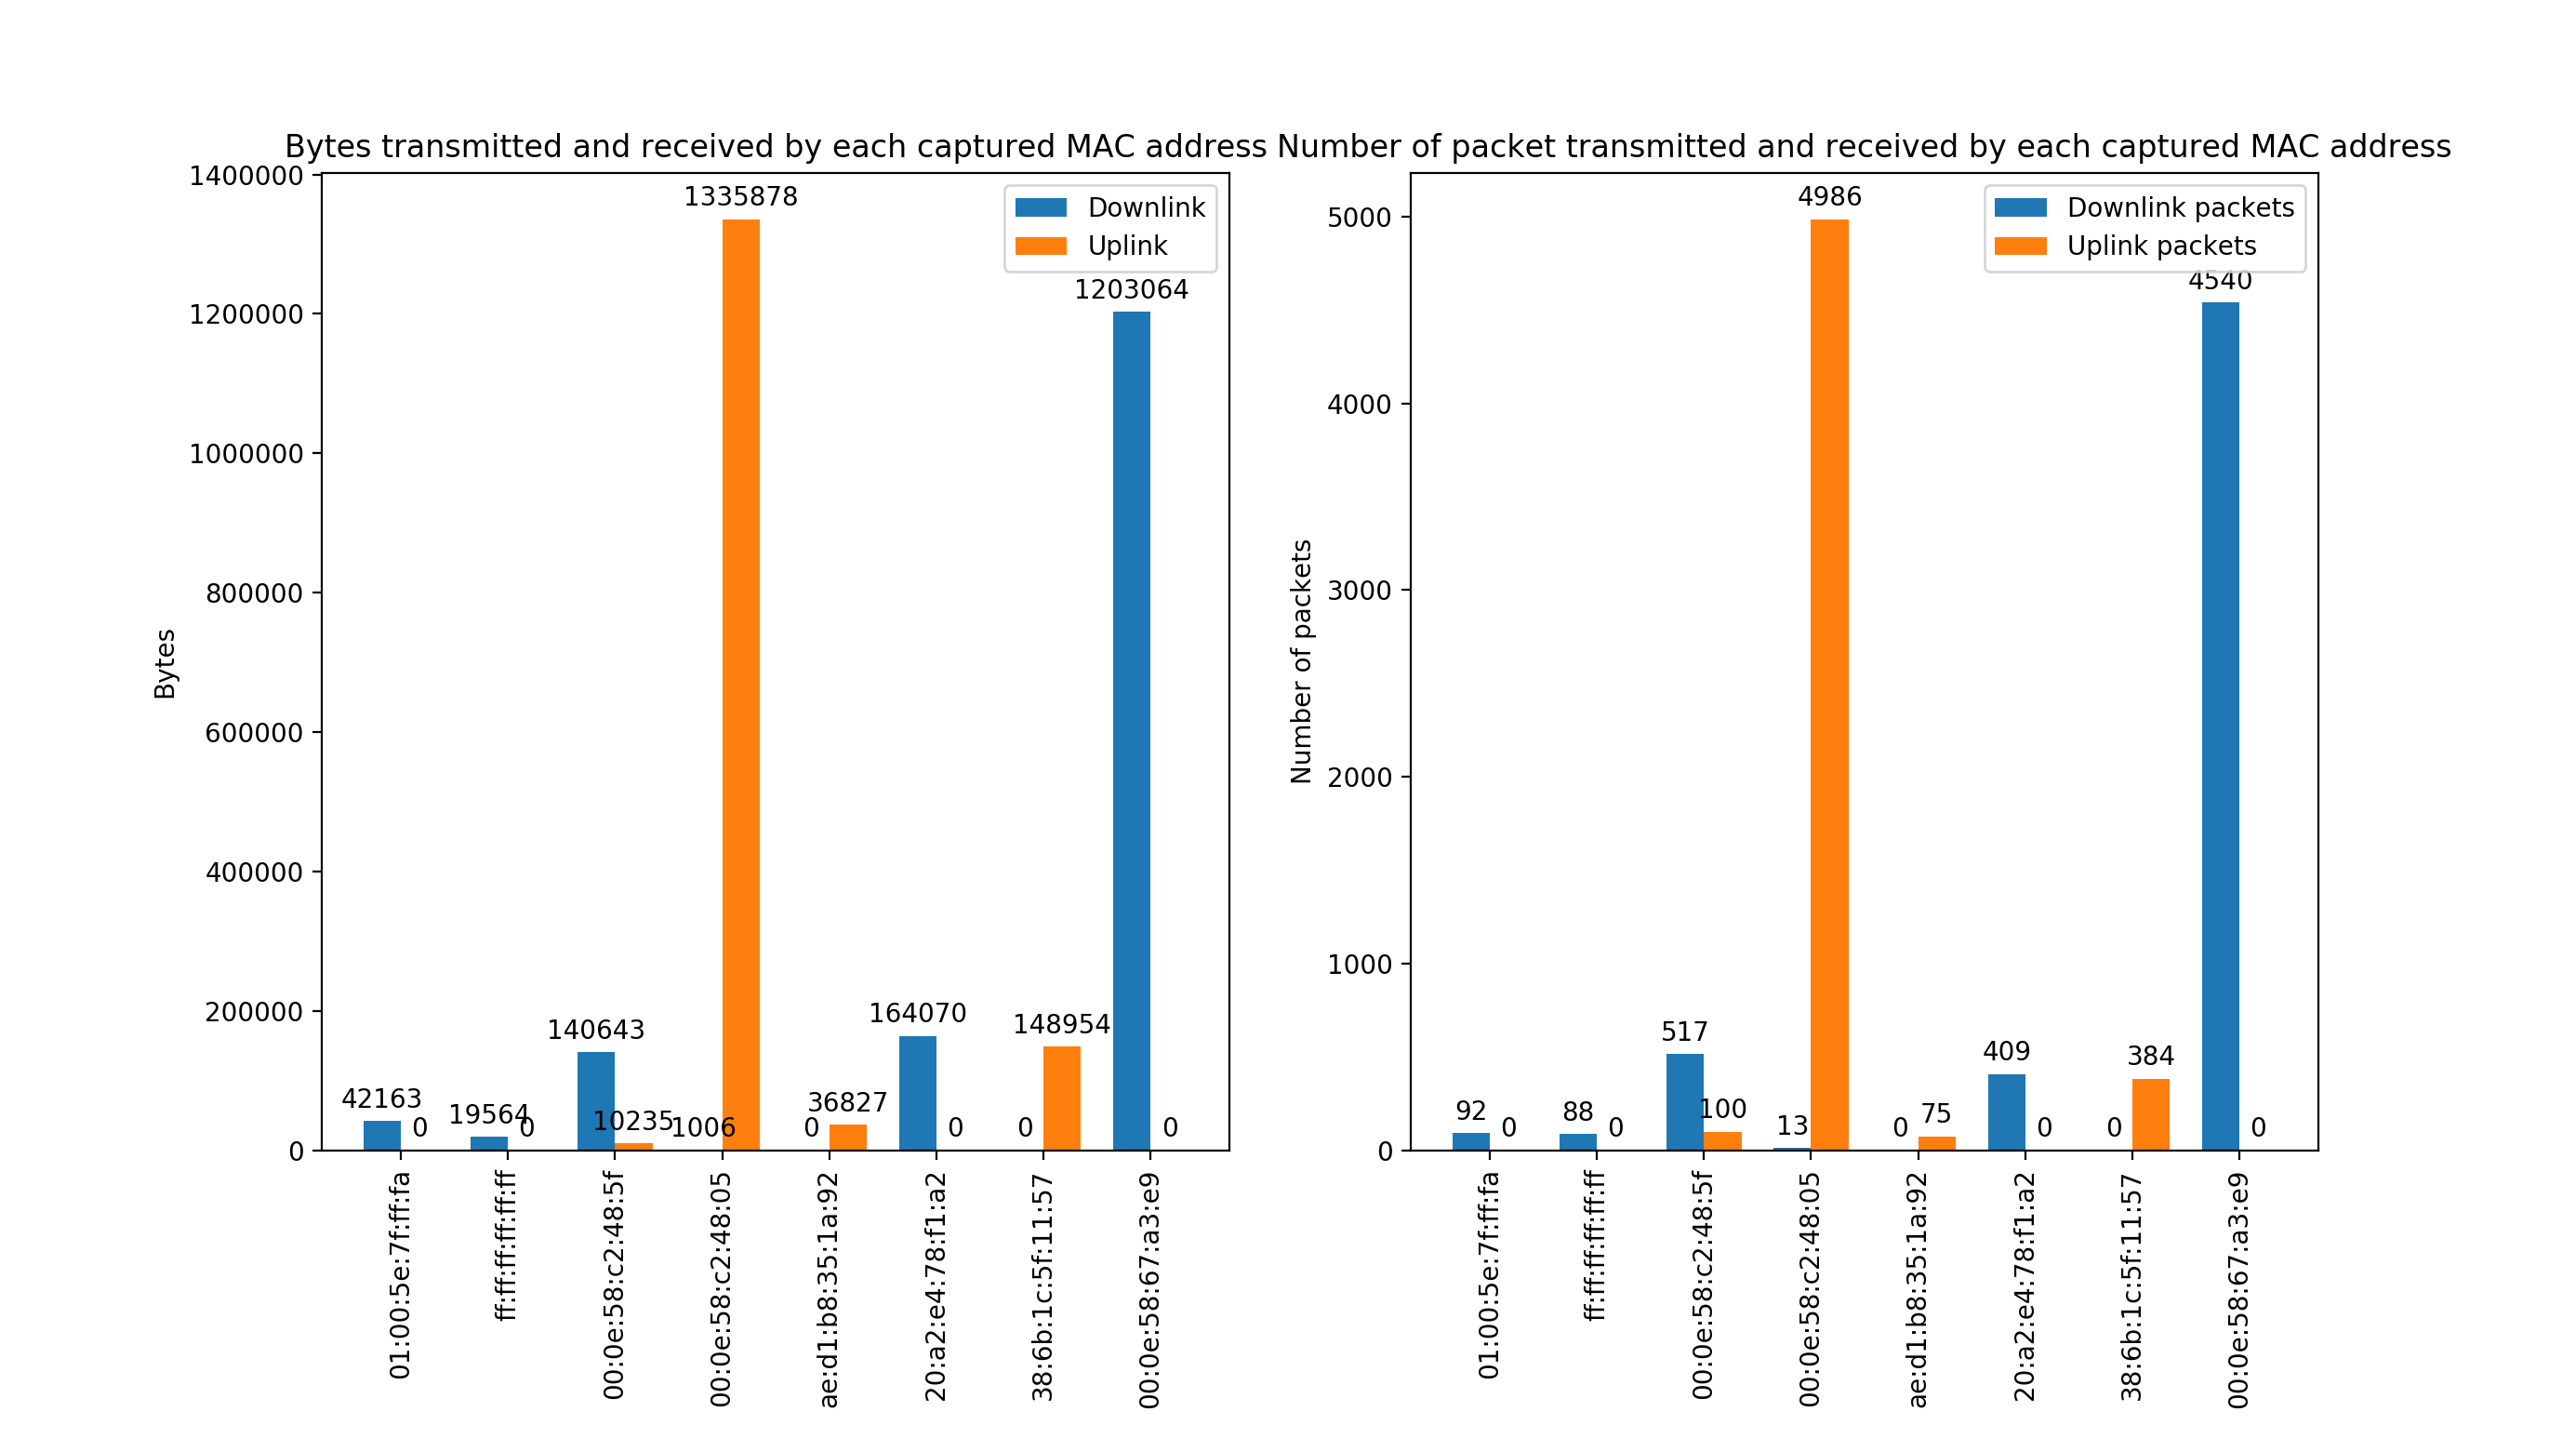
\includegraphics[width=\textwidth]{Graphs/SONOS_bytes_packets.png}
    \caption{Sonos packets exchanged}
    \label{fig:Sonos_packets}
\end{figure}


\subsection{Multimedia internet capture}
In this paragraph, we analyze the results obtained with a capture performed during a lecture of
multimedia internet (\texttt{Multimedia\_internet.pcapng}).
The lecture has been followed using \textit{Microsoft\ Teams}: the professor was presenting the
topic sharing its screen and all the students were following him with their camera and microphone turned off.\\
In Figure \ref{fig:Multimedia internet lecture: data and packets exchanged.}, we can see on the
left the graphs reporting the number of bytes transmitted and received by some of the \textit{MACs}
we have revealed and on the right the number of transmitted and received by the same \textit{MACs}.\\
As we can see, there are some \textit{MACs} that are exchanging much more traffic than others:

\begin{itemize}
    \item \textbf{88:ae:07:3d:8a:30}: this is the device (an \textit{iPad\ Pro}) from which the lecture 
            was being attended. Even if the capture lasted only 5 minutes, we can see that this 
            device has received a lot of bytes (about 42.660 MB): this is of course due to the fact
            that the device was receiving data from a video-conferencing application.\\ 
            If we consider the number of packets received by this \textit{MAC}, we can compute the 
            average length of the packets during the 5 minutes of the capture:

            \begin{equation}
                \textit{Average packet length} = \textit{Number of bytes} / \textit{Number of packets} = 594 Bytes
            \end{equation}

    \item \textbf{20:b0:01:22:22:66}: this is the access point of the home were the lecture was being
            attended. Indeed, we can see that the access point has sent a lot of bytes and packets: 
            most of them were probably destined to the \textit{iPad\ Pro} that was being used to
            follow the lecture since that device was connected to this access point while attending 
            the class. 
\end{itemize}

Among the other \textit{MAC} addresses present in the graph but that have exchanged only a few 
packets in compared with the 2 ones mentioned above, we recognize only \textbf{dc:a9:04:91:42:b9}: 
it's a \textit{MacBook Pro} in the same home. During the 5 minutes of the capture, this device was 
being used for smart-working purposes.

\begin{figure}[h]
    \centering
    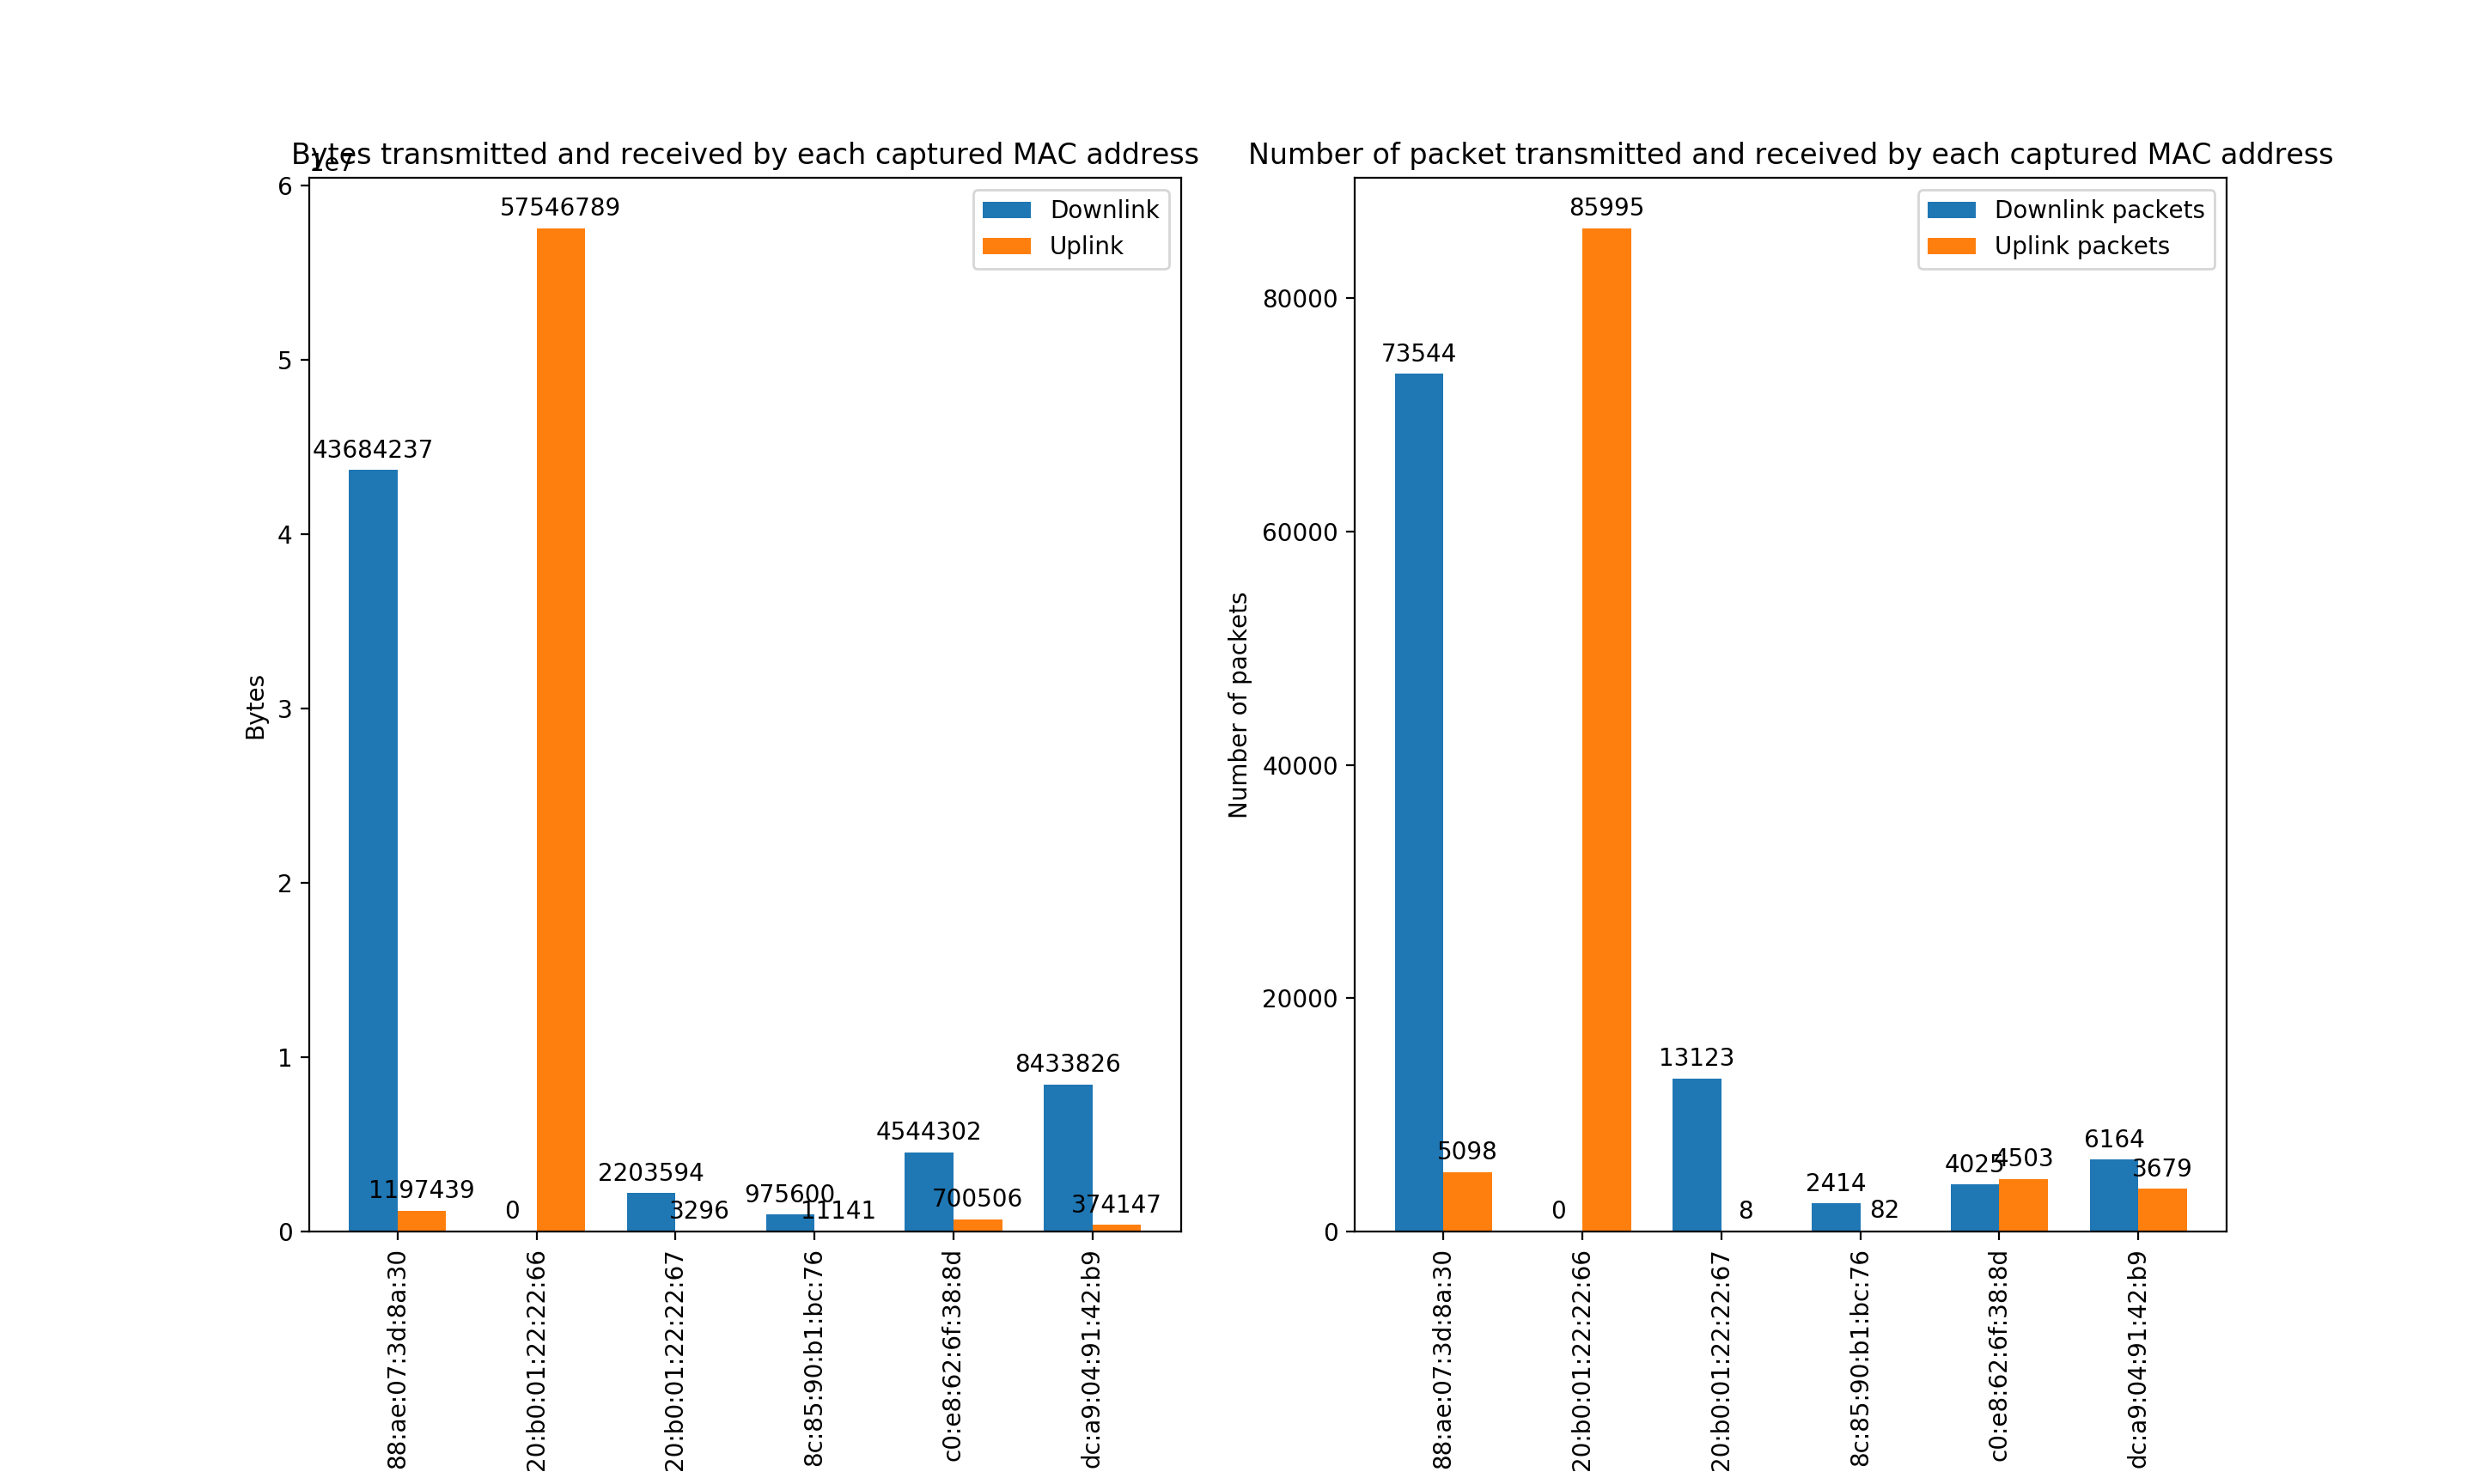
\includegraphics[width=\linewidth]{Graphs/Multimedia_internet_bytes_packets.png}
    \caption{Multimedia internet lecture: data and packets exchanged.}
    \label{fig:Multimedia internet lecture: data and packets exchanged.}
\end{figure}


\subsection{Zoom capture}
In this capture, we were able to see a really big flow of data due to a \textit{Zoom} video call activated from 
one of our known devices.\\ 
As we can see in Figure \ref{fig:Zoom_packets} there are two devices which creates most of the traffic are:
\begin{itemize}
    \item \textbf{8c:85:90:b1:bc:76}: the MacBook from which the call is activated. 
    \item \textbf{20:b0:01:22:22:66}: the router to which the MacBook is connected. 
\end{itemize}
Since all the devices involved were known, we were able to pair the result of the analysis with our 
knowledge on what was really happening at the moment to assign a real meaning to the packets flow 
captured. In this case most of the packets on the client side come from downlink since the client 
has to receive data on video and audio of all the other participants to the call. On the other hand,
the router is sending all those messages to the client so it will register an intense uplink traffic.\\
We can also see that the number of uplink packets in the router is bigger than the number of downlink
packets sent by the MacBook since also other devices were connected to the same network at the same
time. 
\begin{figure}[h]
    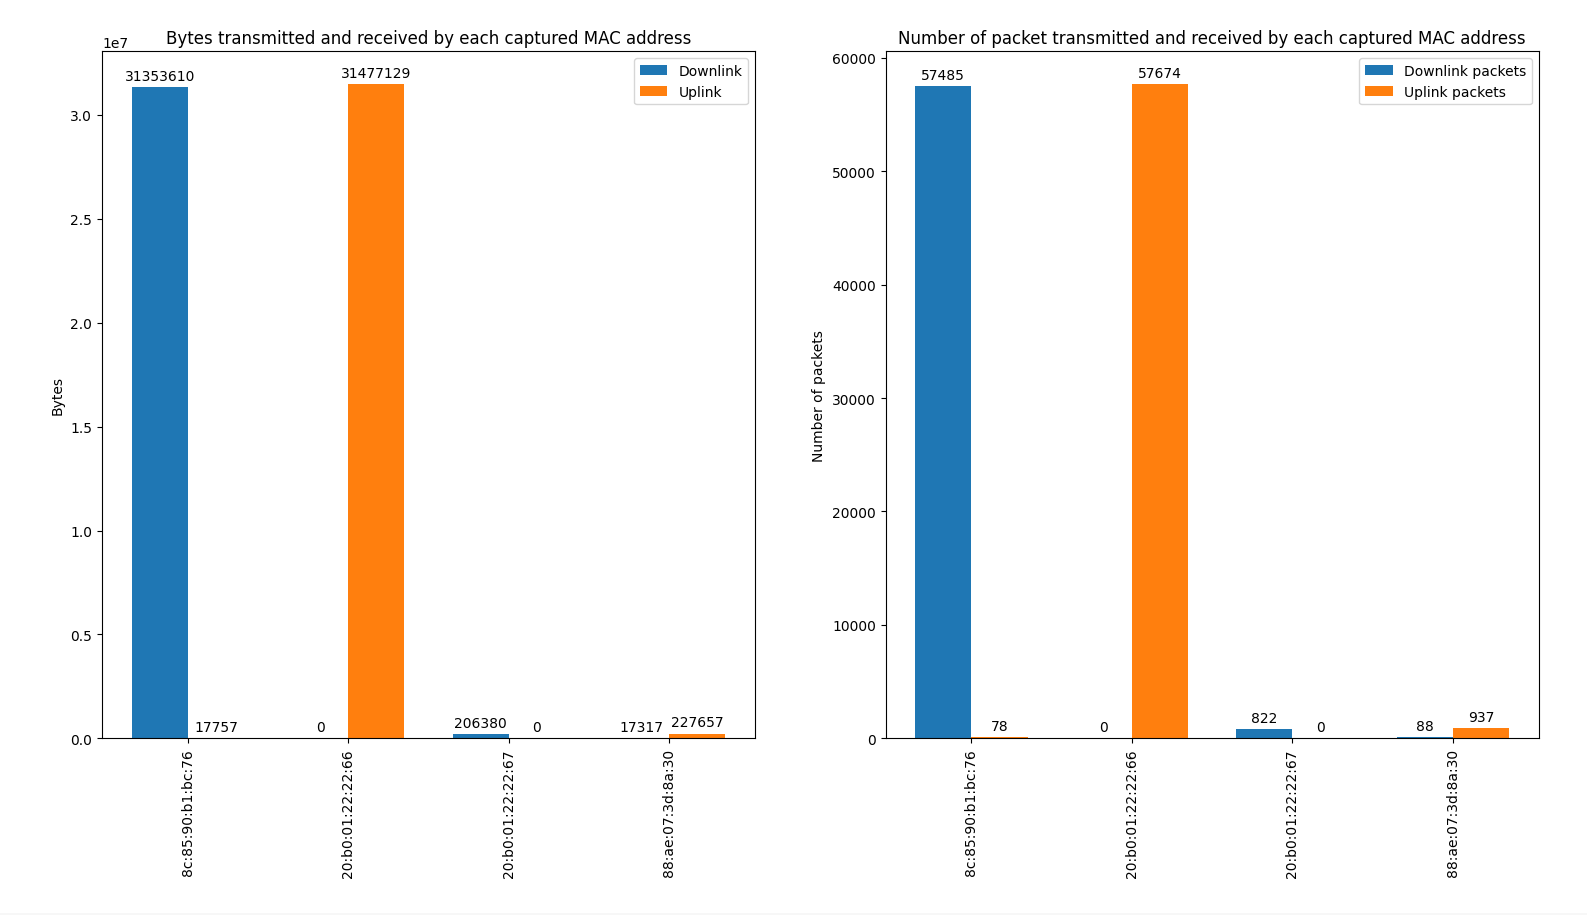
\includegraphics[width=\textwidth]{Graphs/Zoom_bytes_packets.png}
    \caption{Zoom packets exchanged}
    \label{fig:Zoom_packets}
\end{figure}


\subsection{Sunday launch time capture}
In this paragraph, we present the results coming from a capture that has been done in Livorno on a Sunday, in particular at
launch time, from around 1.00 p.m. to 2.35 p.m. (\texttt{Sunday\_launch.pcapng})\\ 
In Figure \ref{fig:Sunday launch packets.}, we can see the amount of bytes (on the left) and packets (on the right)
transmitted and received by the revealed \textit{MACs}. The ones we are able to recognize are:
\begin{itemize}
    \item \textbf{20:b0:01:22:22:66}: the access point of the home where the capture has been performed.
    \item \textbf{88:ae:07:3d:8a:30}: an \textit{iPad\ Pro}.
    \item \textbf{8c:85:90:b1:bc:76}: a \textit{MacBook\ Pro}.
    \item \textbf{c0:e8:62:6f:38:8d}: an \textit{iPhone}.
    \item \textbf{d0:c5:f3:ab:82:63}: another \textit{iPhone}.
    \item \textbf{c0:9a:d0:e4:35:a5}: a third \textit{iPhone}.
\end{itemize}
All of the just mentioned devices belong to users living in the home where we have done the capture, and are the ones the have
exchanged most of the traffic; the other devices are unknown to us.\\
As we can see, the device that has received the highest number of bytes/packets is the access point (\textbf{20:b0:01:22:22:66}),
which also has sent no bytes to any device. \\
Looking at Figure \ref{fig:Sunday launch packets.}, we can also see that 3 of the known devices (\textbf{88:ae:07:3d:8a:30}, 
\textbf{d0:c5:f3:ab:82:63}, \textbf{c0:9a:d0:e4:35:a5}) have sent quite a lot of traffic.\\
Moreover, if we look at Figure \ref{fig:Sunday launch input traffic.}, we can see that the amount of traffic exchanges is very
low for the first (about) 4800 seconds (80 minutes) and that it grows a lot in the last 15 minutes of the capture, so almost all the 
traffic has been sent to the access point mainly from the 3 just mentioned devices in those last 15 minutes.\\
Therefore, what we can conclude is that the owners of the devices haven't used them while having launch and have started 
sending data to the network again once they have finished to eat, which is something very reasonable.\\
For what concerns the other devices, the same reasoning applies to them too, with the difference that they have exchanged only a 
few traffic if compared with the one of the 3 devices mentioned above. 

\begin{figure}[h]
    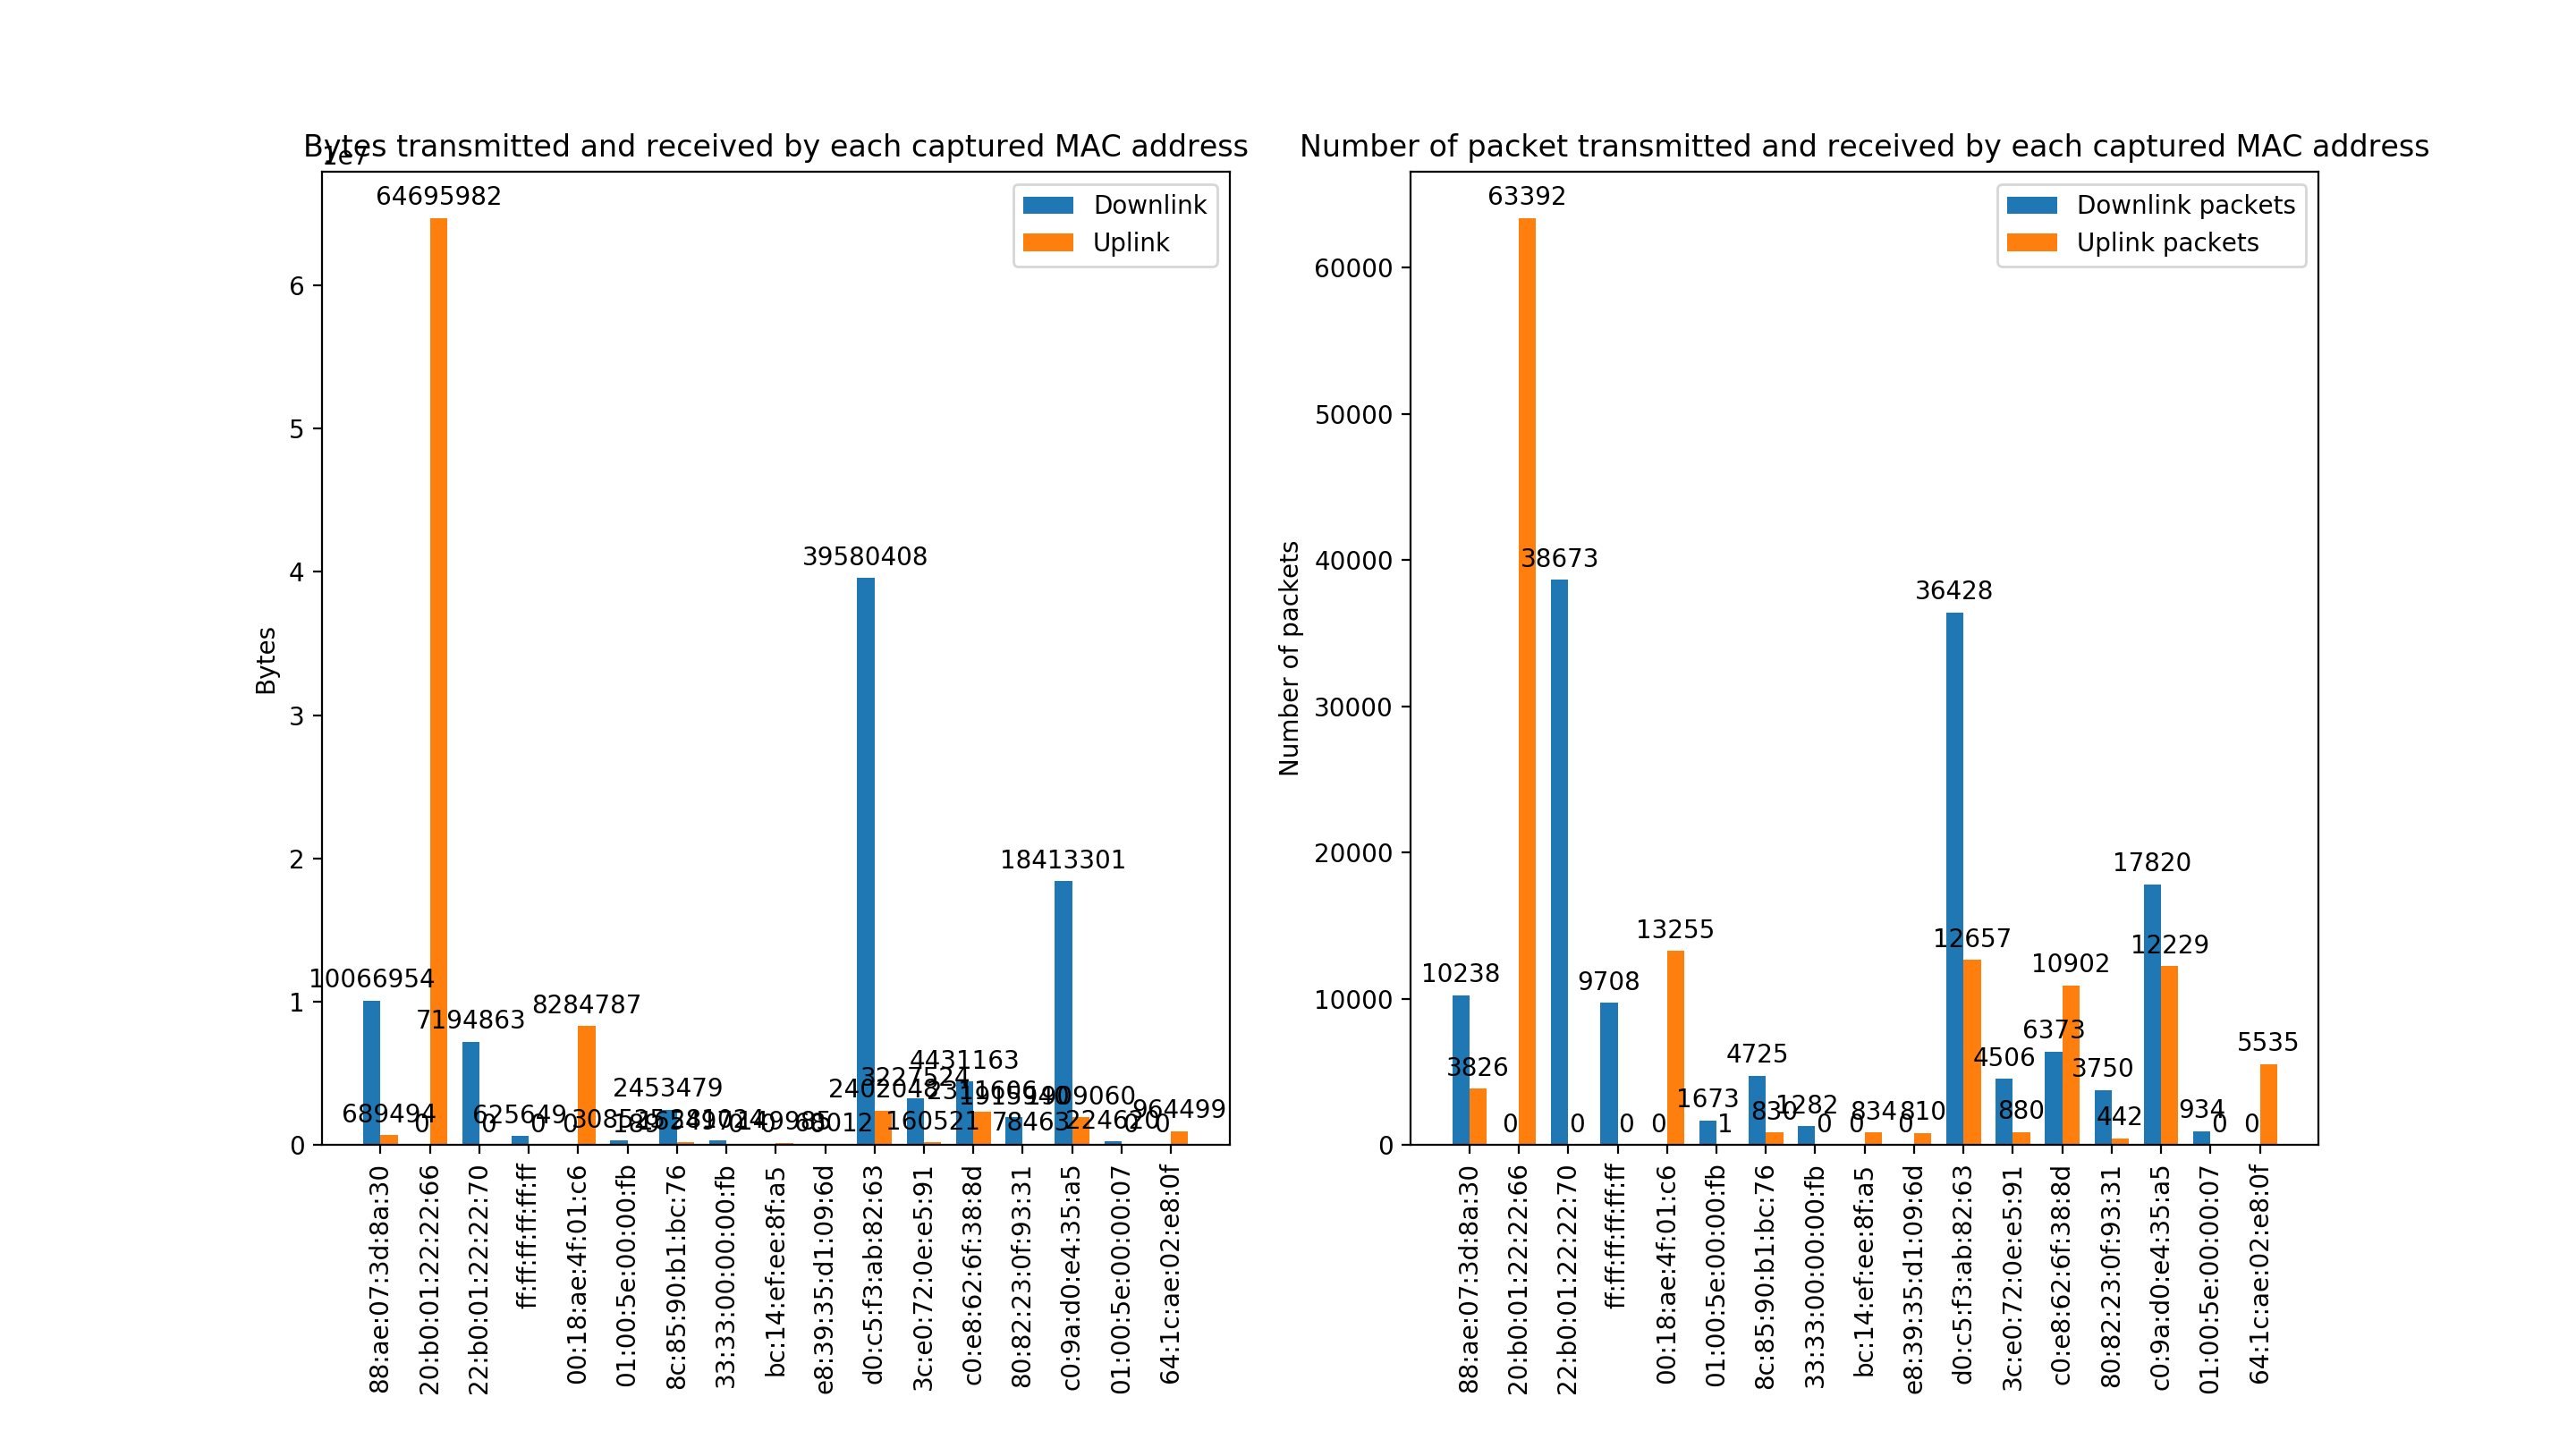
\includegraphics[width=\textwidth]{Graphs/Sunday_launch_bytes_packets.png}
    \caption{Sunday launch packets exchanged.}
    \label{fig:Sunday launch packets.}
\end{figure}

\begin{figure}[h]
    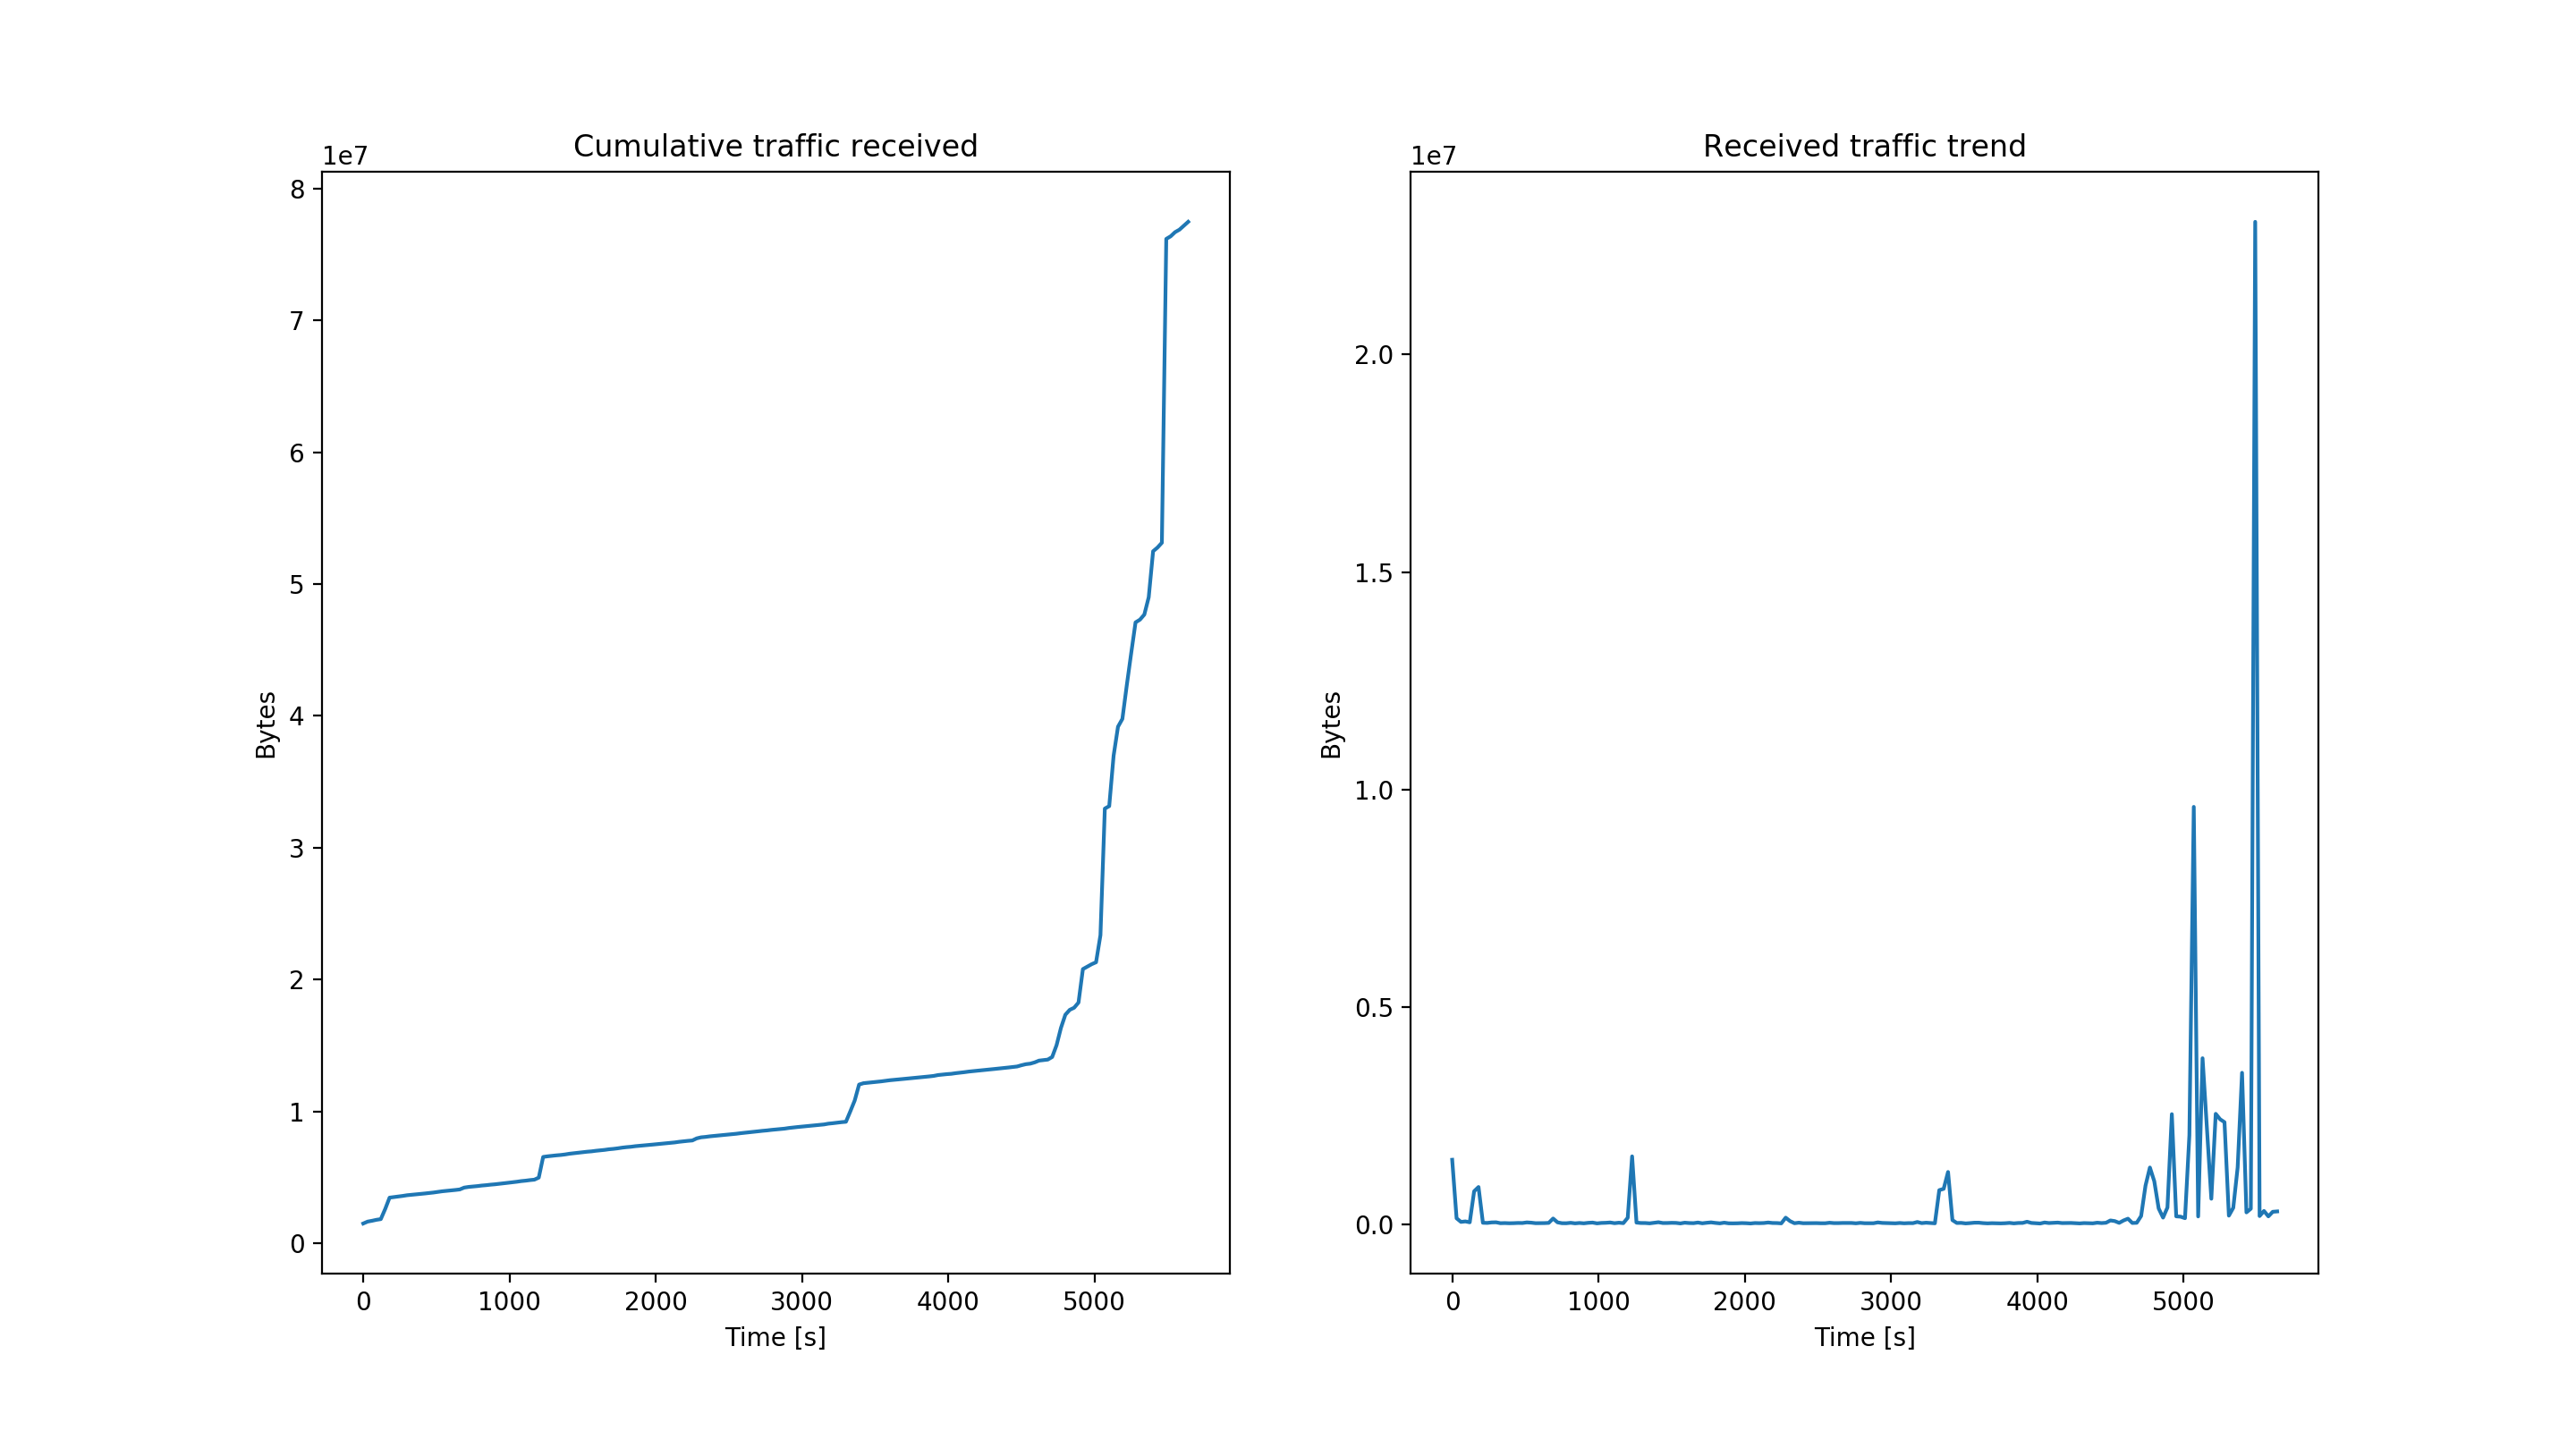
\includegraphics[width=\textwidth]{Graphs/Sunday_launch_cum_in_traffic.png}
    \caption{Sunday launch input traffic.}
    \label{fig:Sunday launch input traffic.}
\end{figure}